\documentclass[conference]{IEEEtran}
\IEEEoverridecommandlockouts
% The preceding line is only needed to identify funding in the first footnote. If that is unneeded, please comment it out.
\usepackage{cite}
\usepackage{amsmath,amssymb,amsfonts}
\usepackage{algorithmic}
\usepackage{graphicx}
\usepackage{textcomp}
\usepackage{xcolor}
\def\BibTeX{{\rm B\kern-.05em{\sc i\kern-.025em b}\kern-.08em
    T\kern-.1667em\lower.7ex\hbox{E}\kern-.125emX}}
\begin{document}

\title{Resolução do Klotski utilizando Métodos de Pesquisa em Python (Tema 1/ Grupo 31)\\
{\footnotesize \textsuperscript{*}Note: Sub-titles are not captured in Xplore and
should not be used}
\thanks{Identify applicable funding agency here. If none, delete this.}
}

\author{\IEEEauthorblockN{André Lopes dos Santos (200505634)}
\IEEEauthorblockA{\textit{Departamento de Engenharia Informática} \\
\textit{Faculdade de Engenharia da Universidade do Porto}\\
Porto, Portugal \\
up200505634@fe.up.pt}
\and
\IEEEauthorblockN{Bernardo Oliveira Teixeira Santos (201504711)}
\IEEEauthorblockA{\textit{Departamento de Engenharia Informática} \\
\textit{Faculdade de Engenharia da Universidade do Porto}\\
Porto, Portugal \\
up201504711@fe.up.pt}
\and
\IEEEauthorblockN{Miguel Rossi  Seabra (200604224)}
\IEEEauthorblockA{\textit{Departamento de Engenharia Informática} \\
\textit{Faculdade de Engenharia da Universidade do Porto}\\
Porto, Portugal \\
ei06054@fe.up.pt}
}

\maketitle

\begin{abstract}
Abordagem a diversos métodos de pesquisa e seus algoritmos, que são uma componente importante da inteligência artificial, assim como à utilização dos mesmos na resolução do Klotski, um conhecido puzzle de deslizamento de blocos.
A linguagem utilizada para a implementação do mesmo é o Python, sendo que o código nesta linguagem para a implementação deste puzzle e para a aplicação dos diferentes algoritmos é adaptado para atingir os objetivos.
\end{abstract}

\begin{IEEEkeywords}
Inteligência Artificial, Pesquisa, Algoritmo A*, Klotski
\end{IEEEkeywords}

\section{Introdução}
Neste trabalho abordar-se-ão diversos métodos de pesquisa em Python aplicados à resolução de puzzles de blocos conhecidos pelo nome “Klotski”, mas mais especificamente a iteração deste que está presente na Google Play Store \cite{b1} Discutir-se-á a história do jogo, as suas regras e a formulação formal do problema. Também falar-se-á dos diferentes métodos de pesquisa, da sua implementação em Python e a eficiência dos mesmos para o jogo em questão. 

\section{Descrição do Problema}
Os puzzles Klotski são puzzles de movimento de blocos em que o objetivo é mover um bloco específico para um sítio específico, movendo todas as outras peças nesse processo. Na Figura \ref{fig:klotski1} pode-se ver um exemplo de um puzzle.

\begin{figure}
	\centering
	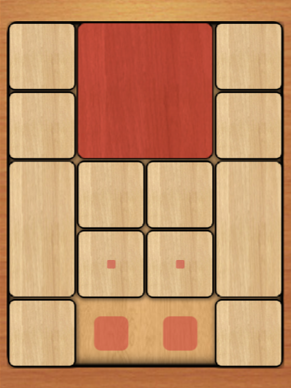
\includegraphics[width=0.75\linewidth]{klotski1.png}
	\caption{Puzzle básico de Klotski, sendo o bloco vermelho aquele que tem de ir para um local específico (pontos vermelhos)}
	\label{fig:klotski1}
\end{figure}

A origem deste puzzle é ainda incerta, mas pensa-se que uma primeira iteração do mesmo tenha sido patenteada por Henry Walton em 1893, embora existam diversos países (Inglaterra, Japão) que reclamam a autoria do puzzle “Original”, sendo que ainda hoje é desconhecida (ou não existe consenso) quanto à origem do mesmo. \cite{b2}
A variante aqui estudada é a iteração presente na Google Play Store \cite{b1} que acrescenta regras como blocos que não se podem mover (i.e. paredes) e outros blocos azuis que se portam como paredes até que o bloco vermelho toque em todos eles, fazendo-os desaparecer. Na Figura \ref{fig:klotski2} pode-se ver um exemplo de um puzzle que contém paredes (representadas por blocos castanhos) e os já mencionados blocos azuis.


\begin{figure}
	\centering
	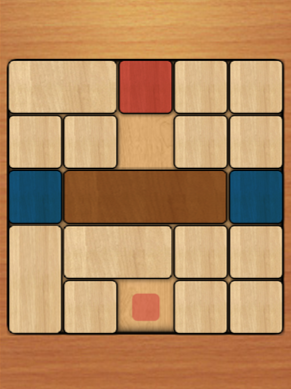
\includegraphics[width=0.75\linewidth]{klotski2.png}
	\caption{Puzzle de Klotski com paredes (representado com blocos castanhos) e com blocos azuis.}
	\label{fig:klotski2}
\end{figure}



\section{Formulação do Problema}
\textbf{Representação do Estado:} O estado é representado por uma Matriz de tamanho variável (a * b) [0 – espaço livre], e pela posição das diferentes peças que são numeradas (1, 2, 3, etc.). 
Tanto as células do puzzle como os as diferentes peças, têm uma característica extra: n- normal; f-final. No caso das células estes representam as células normais do jogo enquanto as células finais representam os sítios onde se devem encontrar as peças finais. No caso das diferentes peças, as peças normais representam as peças móveis que se conhecem, e a peça final é aquela cujo objetivo é levar à(s) célula(s) final(ais).

\textbf{Estados Iniciais:} Os estados iniciais variam conforme o puzzle a ser resolvido. Na Figura 1 pode-se ver um exemplos de uma representação gráfica de um estado inicial de um puzzle. Na Figura 3 pode-se ver uma representação desse mesmo puzzle num terminal.

\begin{figure}
	\centering
	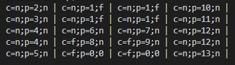
\includegraphics[width=0.75\linewidth]{klotski3.png}
	\caption{Puzzle de Klotski: Representação no terminal}
	\label{fig:klotski3}
\end{figure}

\textbf{Teste Objetivo:} A peça final deverá chegar à localização das células finais e chegar lá no número mínimo de jogadas possível.

\textbf{Operadores/Jogadas:} Mov(N,D) – Movimentação da peça N (sendo N um número acima de 1 mas igual ou inferior ao número mais alto),na direcção D (Cima, Baixo, Esquerda ou direita).

\textbf{Pré-condições:} Uma peça possa mover-se na direção desejada, i.e. ter espaço livre para todos os elementos da peça se poderem mover na direção desejada.

\textbf{Efeitos:} Mov(1, Cima) – A peça 1 move-se (se possível) uma casa para cima.



\section{Trabalho Relacionado}
Foram encontradas diversas implementações em Python do puzzle Klotski, algumas com solvers já implementados \cite{b3} \cite{b4} \cite{b5} \cite{b6} \cite{b7}. A implementação do Klotski será baseada nestas mesmas fontes, sendo que serão realizadas diversas adaptações ao caso específico deste trabalho.
Os métodos de pesquisa utilizados serão pesquisa em largura, pesquisa em profundidade, aprofundamento progressivo, custo uniforme, pesquisa gulosa e Algoritmo A*, sendo a implementação destes métodos baseados naqueles presentes no livro “Artificial Intelligence: A Modern Approach” (sendo este o livro principal da cadeira de Inteligência Artificial) \cite{b8}, sendo que o código (em várias linguagens) para a implementação destes algoritmos está disponível online \cite{b9}.

\section{Implementação do Jogo}
Como foi referido anteriormente, foram encontradas diversas implementações do jogo realizadas por diversas pessoas diferentes, no entanto a implementação do jogo que foi utilizada foi uma criada de raíz, sendo que as outras implementações encontradas serviram apenas como elemento de consulta quando necessário.
O Programa utiliza ficheiros csv como meio para "receber" o estado do puzzle, seu tamanho, localização das diferentes peças e local final (onde deve ficar a peça objetivo).
Tendo o estado do puzzle e o seu objetivo final, são aplicados os diferentes métodos de pesquisa para saber quais os passos necessários para chegar ao estado final no menor tempo possível.


\section{Algoritmos de Pesquisa}
Foram implementados os diferentes algoritmos de pesquisa para proceder à resolução deste puzzle. Os algoritmos implementados foram: Pesquisa Primeiro em Largura ("Breadth-First Search"), Pesquisa de Custo Uniforme, Pesquisa Primeiro em Profundidade ("Depth-First Search"), Pesquisa em Profundidade Iterativa, Pesquisa Gulosa ("Greedy Search") e Pesquisa A*. Para implementar estes diferentes algoritmos no nosso jogo, foi adaptado a lógica de jogo aos algoritmos do livro \cite{b8}, sendo que o código desses mesmos algoritmos é o mesmo presente no GitHub do livro \cite{b9}.


\section{Experiências e Resultados}
Realizaram-se diversas experiências, comparando o desempenho dos diferentes algoritmos na resolução dum puzzle Klotski. Na tabela seguinte pode-se ver a comparação dos diferentes métodos de resolução

\begin{table}[htbp]
\caption{Comparação dos diferentes métodos de pesquisa}
\begin{center}
\begin{tabular}{|c|c|c|}
\hline
\textbf{Método de pesquisa} & \textbf{Tempo (segundos)} & \textbf{Número de nós)} \\
\hline
 Pesquisa Primeiro em Largura & 23 & 45\\
 Pesquisa de Custo Uniforme & 23 & 45 \\
 Pesquisa Primeiro em Profundidade & 23 & 45\\
 Pesquisa em Profundidade Iterativa & 23 & 45\\
 Pesquisa Gulosa & 23 & 45\\ 
 Pesquisa A* & 23 & 45\\
\hline

\end{tabular}
\label{tab1}
\end{center}
\end{table}


\section{Conclusões e Perspetivas de Desenvolvimento}
Como se pode verificar na secção anterior, e tal como seria teoricamente esperado, o método A* foi aquele que mostrou ser o mais eficaz na resolução do puzzle klotski. Infelizmente ainda não foi possível implementar certas regras de jogo que são específicas em relação ao que existe na Google Play Store.






\section*{Referências Bibliográficas}



\begin{thebibliography}{00}
\bibitem{b1} “Klotski - Aplicações no Google Play,” [Online]. Available: https://play.google.com/store/apps/details?id=com.alcamasoft.juegos.klotski.android. [Acedido em 15 03 2019].
\bibitem{b2} “Klotski - Wikipedia,” [Online]. Available: https://en.wikipedia.org/wiki/Klotski. [Acedido em 06 03 2019].
\bibitem{b3} Goshuujin, “Github - Goshuujin/Klotski,” [Online]. Available: https://github.com/Goshuujin/Klotski. [Acedido em 16 03 2019].
\bibitem{b4} SamuelDSR, “Github - SamuelDSR/Klotski-python,” [Online]. Available: https://github.com/SamuelDSR/Klotski-python. [Acedido em 16 03 2019].
\bibitem{b5} aschmied, “Github - aschmied/klotski-solver,” [Online]. Available: https://github.com/aschmied/klotski-solver. [Acedido em 16 03 2019].
\bibitem{b6} jwmullally, “Github - jwmullally/klotski\_solver,” [Online]. Available: https://github.com/jwmullally/klotski\_solver. [Acedido em 16 03 2019].
\bibitem{b7} D. R. Ying Dang, “Github,” [Online]. Available: https://github.com/whydang/klotski.
\bibitem{b8}  S. Russel e P. Norvig, Artificial Intelligence: A Modern Approach, Pearson Education Inc., 2010.
\bibitem{b9} S. Russel e P. Norvig, “AimaCode - Code for the Book Artificial Inteligence: A Modern Approach",” 2019. [Online]. Available: https://github.com/aimacode. [Acedido em Março 2019].


\end{thebibliography}
\vspace{12pt}
\color{red}

\end{document}
